\documentclass[12pt]{article}
\usepackage[pdftex]{rotating}
\usepackage{amsmath,amsthm}
%\usepackage[pdftex]{graphicx}
%\usepackage[abbr]{harvard}
%\usepackage[margin=1in]{geometry}
\usepackage{booktabs}
\usepackage{setspace}
\usepackage{hyperref}

\pdfpagewidth 8.5in
\pdfpageheight 11in

\setcounter{secnumdepth}{3}

\title{Distributed Batch Runs in Repast Simphony}


\begin{document}

\begin{titlepage}
\maketitle
\vfill
%\vspace{.5in}

\thispagestyle{empty}
\end{titlepage}

\pagebreak

\section{Developing a Distributed Batch Repast Simphony Project}

A new feature within Repast Simphony is a largely automated distributed batch framework that allows users to distributed their
simulations in batch mode using multiple computer nodes and/or cores. This feature takes advantage of Repast Simphony's previous
batch development but adds a new layer of capability in a plugin called repast.simphony.distributedBatch. The instructions below detail
how users can setup their own distributed batch process using a Predator Prey project example. Previous Repast capability in allowing
users to conduct single node batch runs are still enabled
in the 2.0 version of Repast Simphony. This is done, as in previous
versions of Repast Simphony, in
the repast.simphony.batch plugin.
\subsection{Downloading and Installing GridGain}
The first step in using distributed batch for your project is to go to
the GridGain website (\hyperlink
{http://www.gridgain.com/}{http://www.gridgain.com/}) and download
GridgGain 2.1.1 at: \hyperlink
{http://www.gridgain.com/past_downloads.html}
{http://www.gridgain.com/past\_downloads.html}. Repast Simphony is
currently using GridGain 2.1.1 because during the time of development
this was the stable version released by GridGain. In addition, a new
licensing scheme by GridGain makes the 2.1.1. version more feasible
for Repast Simphony than the newer GridGain 3.0 version. For now, the GridGain 2.1.1 version should work well on
Windows (Windows 2000 and up), Mac (Mac OS X versions), and Linux
systems. Users will need to install GirdGain 2.1.1 on all nodes,
including the computer that they are using to launch Repast Simphony
simulations (Figure 1). Users should read the GridGain 2.1.1 installation
instructions for proper configuration of GridGain 2.1.1. Once
installed, place the repast.simphony.batch.jar, which is found in
the /transferFiles folder of the repast.simphony.distributedBatch
plugin, into the /libs/ext folder located within the GridGain
installation folder (i.e., [location of the GridGain 2.1.1
folder]/libs/ext) for all nodes that have GridGain installed and those
that will be used for distributed Repast batch runs.
\begin{figure}[!t]
\begin{center}
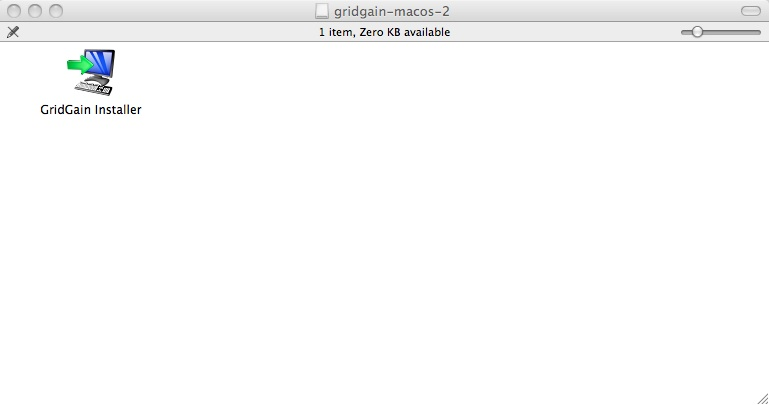
\includegraphics[width=\textwidth] {images/Figure1.jpg}
\label{cablehealth}
\begin{minipage}{.9\textwidth}Figure 1. The GirdGain 2.1.1 installer
  for Mac OS X.
\end{minipage}
\end{center}
\end{figure}

The default-spring.xml file, found in
repast.simphony.distributedBatch, should be used to replace the
default-spring.xml file in the /config folder within the GridGain
2.1.1 installation folder on all nodes used (Figure 2). This file will allow the default
distributed configuration on all nodes used to be the same as that
found in the
repast.simphony.distributedBatch folder, which controlles the
configuration of the user's computer where processes are launched
from.

\begin{figure}[!t]
\begin{center}
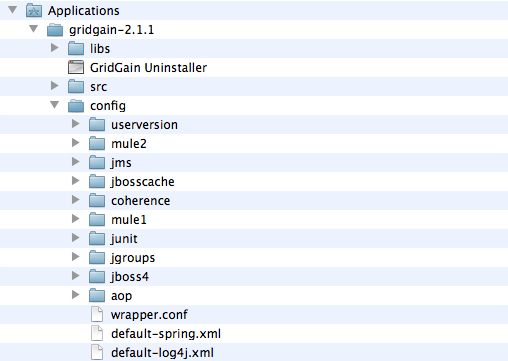
\includegraphics [width=\textwidth]{images/Figure2.jpg}
\label{cablehealth}
\begin{minipage}{.9\textwidth}Figure 2. The default-spring.xml file in
  the /config folder of the GridGain installation
  that should be replaced by the default-spring.xml found in the
  distributedBatch plugin.
\end{minipage}
\end{center}
\end{figure}

\section{Creating the Batch Setup Files}

The next step is creating a standard batch file, often called
batch\_params.xml, which contains the simulation parameters and number
of batch runs (see Repast Simphony's instructions for regular batch
runs). However, because the project is a distributed batch project,
users should set the ``sweep runs'' setting to 1, as the sweep setting
will now be handled by the distributed process. If a user desires to
run a regular batch run (i.e., using only one node), then the user
should set the sweep runs setting to whatever number he or she
desires. The figure (Figure 3) below shows what a standard
batch\_params.xml file looks like. This file should be placed
somewhere within the user's Repast project folder. The
predator\_prey\_batch folder, in the repast.simphony.demo.predatorprey
example project contains, contains the batch\_params.xml file shown in
Figure 3. The user should also remember to setup outputs as they normally would for Repast Simphony projects (e.g., text file outputters).

\begin{figure}[!t]
\begin{center}
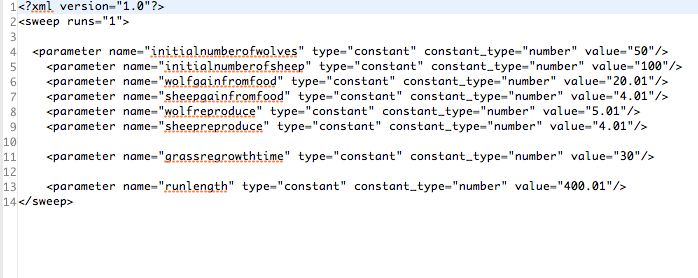
\includegraphics[width=\textwidth]{images/Figure3.jpg}
\label{cablehealth}
\begin{minipage}{.9\textwidth}Figure 3. The standard batch\_params.xml file.
\end{minipage}
\end{center}
\end{figure}

\section{Creating the Project Jar File}

The user then has two options in creating a project jar file to be
used in the distributed runs. The first option is to use tools within
the Eclipse Repast Simphony IDE. In this option, the user needs to
click on their project and create a jar file by choosing File $\rightarrow{}$ Export$ \rightarrow{}$ JAR file.

Then, in the ``Jar Export'' window (Figure 4), name the project jar
and export it. The user will then need to place this jar file in the
/transferFiles folder located in their project folder (e.g.,
see the /transferFiles folder in repast.simphony.demo.predatorprey).

\begin{figure}[!t]
\begin{center}
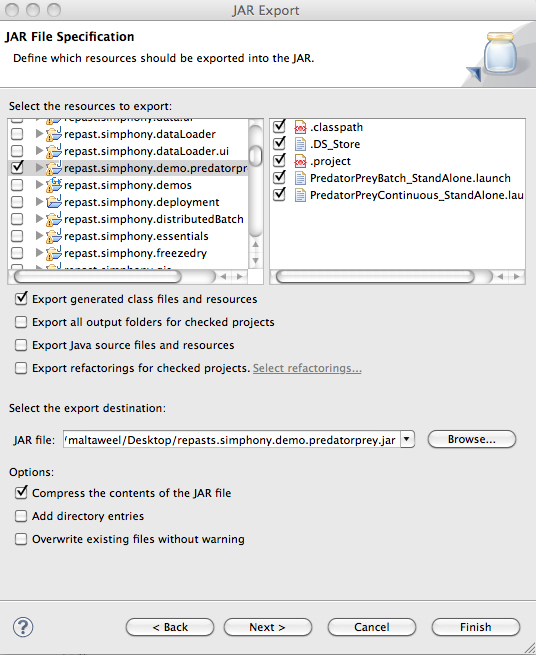
\includegraphics [width=\textwidth]{images/Figure4.jpg}
\label{cablehealth}
\begin{minipage}{.9\textwidth}Figure 4. Jar exporting tool in the Repast Simphony Eclipse IDE.
\end{minipage}
\end{center}
\end{figure}

The second option is to let the repast.simphony.distributedBatch
plugin to automatically build the distributed jar at runtime. This is
done via the build.xml ant file located in the
repast.simphony.distributedBatch plugin. For this case, the user
should have to do nothing aside from configuring the
XML\_Launch\_Inputs.xml file, which has to be configured anyway, and
will be discussed below.

\section{Setting the Distributed Batch Runs}

Next, the user sets up a project that uses the
repast.simphony.distributedBatch plugin. There are several path
settings that need to be determined for both the local node (i.e., the
computer you are using to launch the process) and the remote
nodes. First, look at the XML\_Launch\_Inputs.xml file located in the
/launchData folder within the repast.simphony.distributedBatch
plugin. You will need to edit the following sets of paths and data
(Figures 5 \& 6):

\begin{figure}[!t]
\begin{center}
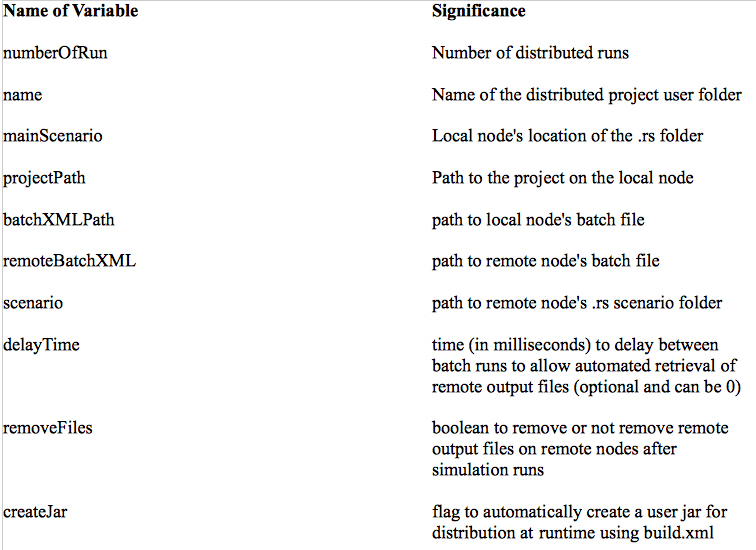
\includegraphics [width=\textwidth]{images/Figure5.jpg}
\label{cablehealth}
\begin{minipage}{.9\textwidth}Figure 5. The XML\_Launch\_Inputs.xml file's user inputs.
\end{minipage}
\end{center}
\end{figure}

\begin{figure}[!t]
\begin{center}
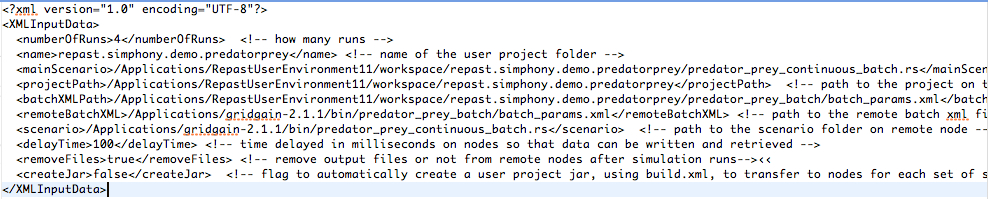
\includegraphics [width=\textwidth]{images/Figure6.jpg}
\label{cablehealth}
\begin{minipage}{.9\textwidth}Figure 6. What the XML\_Launch\_Inputs.xml file looks like.
\end{minipage}
\end{center}
\end{figure}

Repast Simphony applies a ``user\_path.xml'' file that is typically
located in the user's .rs folder (see
repast.simphony.demo.predatorprey as an example). This file allows
Repast Simphony to loaded necessary classes for simulation runs and is
used for regular GUI simulations, regular batch simulation, and
distributed batch runs. In addition to setting the local bin folder's
location, the user needs to indicate where the remote nodes' class bin
folder will be located. In the repast.simphony.distributedBatch
plugin, the processes will launch on the remote nodes from GridGain's
installation /bin folder. When a distributed processes is launched,
the user's .jar project file will be unjared, exposing the class files
in the jar file. The class files will be typically located in the
GridGain /bin folder at that point. Thus, users will need to indicate
a path where the users' classes are located in GridGain. Typically,
the user should place a class reference to the GridGain bin folder (Figure
7). However, if the jar was created via the ant build.xml file, then
they may need to reference their project's bin folder within the bin
of GridGain (Figure 8).

\begin{figure}[!t]
\begin{center}
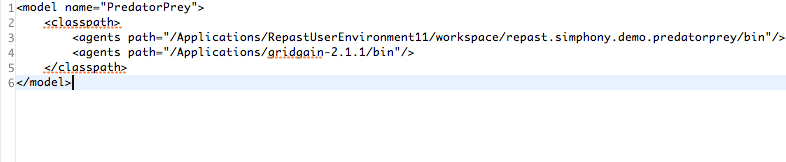
\includegraphics [width=\textwidth]{images/Figure7.jpg}
\label{cablehealth}
\begin{minipage}{.9\textwidth}Figure 7. The reference to the remote
  bin folder seen for projects using the Eclipse jar creator.
\end{minipage}
\end{center}
\end{figure}

\begin{figure}[!t]
\begin{center}
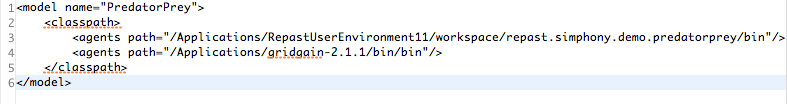
\includegraphics [width=\textwidth]{images/Figure8.jpg}
\label{cablehealth}
\begin{minipage}{.9\textwidth}Figure 8. The reference to the remote
  bin folder seen for projects using ant build.xml file. The two /bin
  references are needed because the user's jar has its own bin folder.
\end{minipage}
\end{center}
\end{figure}

\section{Launching the Remote Nodes}

The user is now ready to launch the remote nodes. First, be sure to
have the JAVA\_HOME and GRIDGAIN\_HOME variables set on the remote
nodes, as stated by the GridGain installation instructions (please
read the GridGain 2.1.1 instructions prior to using GridGain in
Repast). To launch GridGain, simply login into your remote nodes and
launch the ``gridgain.sh'' file or ``gridgain.bat'' file (.sh for Mac and
Linux and .bat for Windows machines). For Mac and Linux machines, type
``sh [path to gridgain.sh file]/gridgain.sh'' in the line command on
the remote node, which should then activae your remote node. For
Windows machines, just type the following path ``[path to gridgain.bat
file]/gridgain.bat'' to do the same process as the other operating
systems. Once launched, you do not need to turn off any nodes if you plan
on running multiple sets of distributed batch runs. However, if any
launch errors occur on the remote nodes or you edit your code, then you will
need to restart the remote nodes as the new classes or updated classes
will need to be reloaded on the remote machines. You may also want to
configure a startup script that will automatically launch your
GridGain startup files on the remote nodes. Once launched, you should
see the remote nodes producing log information that indicates they are
ready to receive processes launched from your local computer and can
connect to other nodes in a cluster (Figure 9).

\begin{figure}[!t]
\begin{center}
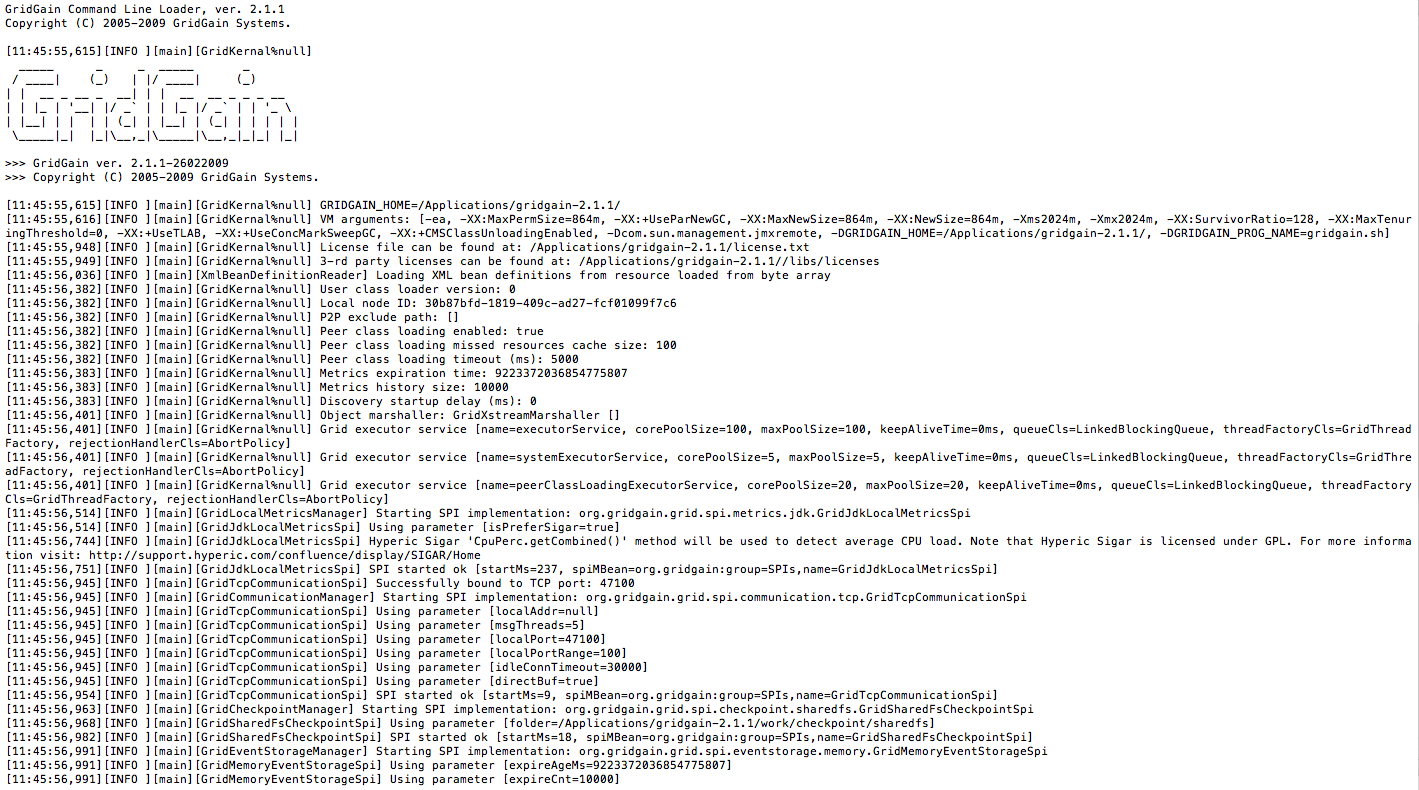
\includegraphics [width=\textwidth]{images/Figure9.jpg}
\label{cablehealth}
\begin{minipage}{.9\textwidth}Figure 9. The remote node launched.
\end{minipage}
\end{center}
\end{figure}

\section{Launching the Distributed Process}

The user can now launch the distributed process. To do this, go to Run
Configurations... in the Repast Simphony Eclipse IDE and in the
run configurations window select the Java Application setup for
BatchMainSetup. There, choose the Classpath tab in the Run
Configurations window. Add the local user project's bin folder to the
User Entries (Figure 10). Then, in the Environment tab edit the local
path to the “GRIDGAIN\_HOME” directory of the GridGain installation
folder (Figure 11). This will automatically startup your local GridGain
application at runtime. Users can also create their own Run
Configurations... setup using similar
settings to the ``'BatchMainSetup.launch'' file located in the
Repast Simphony distributedBatch plugin folder. 

\begin{figure}[!t]
\begin{center}
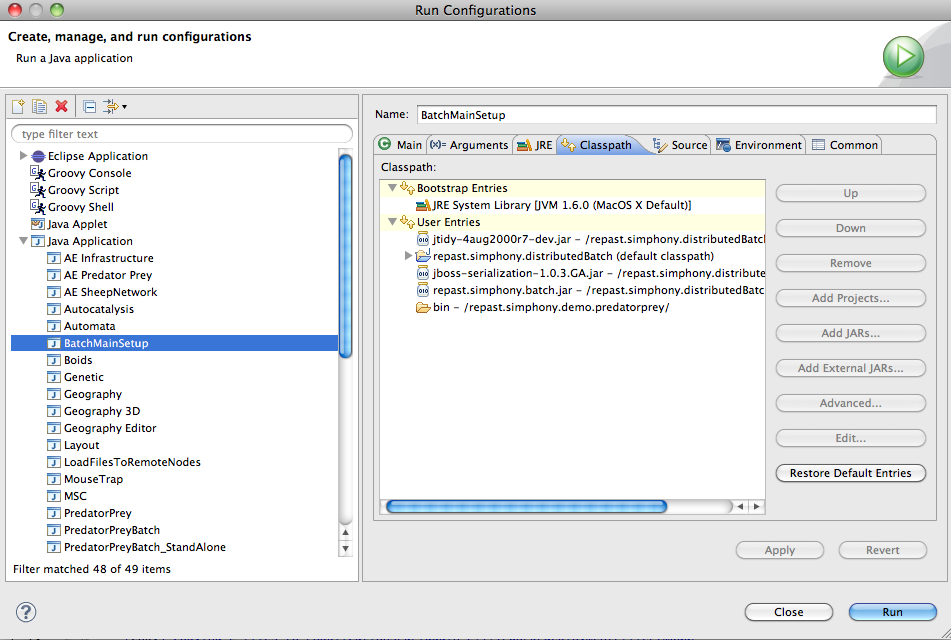
\includegraphics [width=\textwidth]{images/Figure10.jpg}
\label{cablehealth}
\begin{minipage}{.9\textwidth}Figure 10. Reference to the local bin folder.
\end{minipage}
\end{center}
\end{figure}

\begin{figure}[!t]
\begin{center}
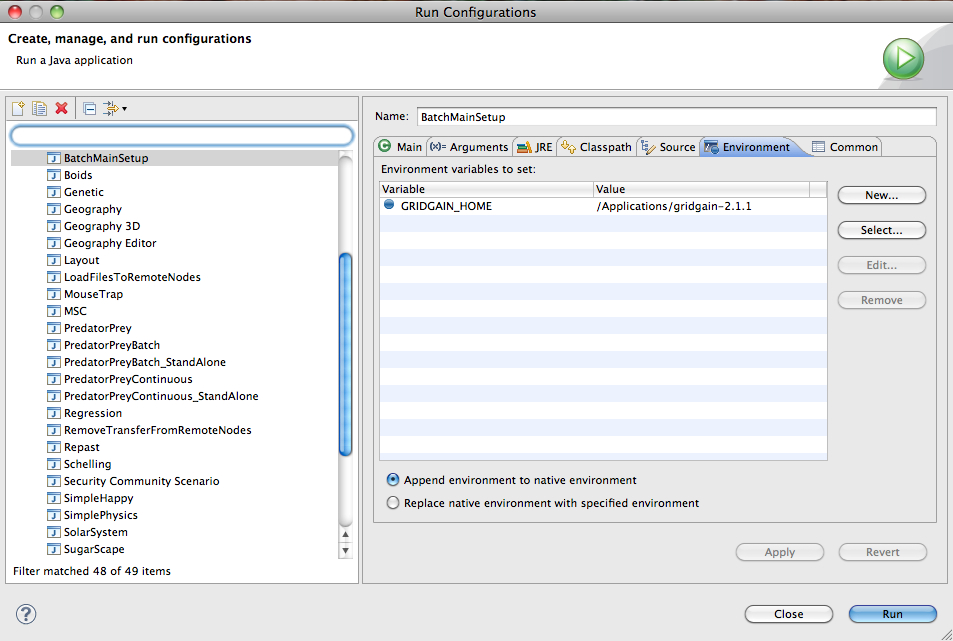
\includegraphics [width=\textwidth]{images/Figure11.jpg}
\label{cablehealth}
\begin{minipage}{.9\textwidth}Figure 11. Environment reference to the
  GridGain installation folder.
\end{minipage}
\end{center}
\end{figure}

Now, the user can select the Run button in the Run Configurations
window (bottom right corner in Run Configurations) and launch the distributed process. The
log should produce output information in the local console window
(Figure 12) and remote nodes (Figure 13), showing the distributed
process running. The output should include information on the number
of nodes running in GridGain and any output console information
produced by the user's project (e.g., in the Predator Prey example the
outputter, setup in the Repast GUI environment, displays user
output). You should also see unique threads running on the local and
remote nodes. The example Predator Prey project (Figures 12 and 13)
shows two nodes (i.e., two computers) executing the model. Another featured in
distributed batch is that it uses automatic failover, which allows
other nodes to take the jobs from machines that may fail during the
batch process. 

\begin{figure}[!t]
\begin{center}
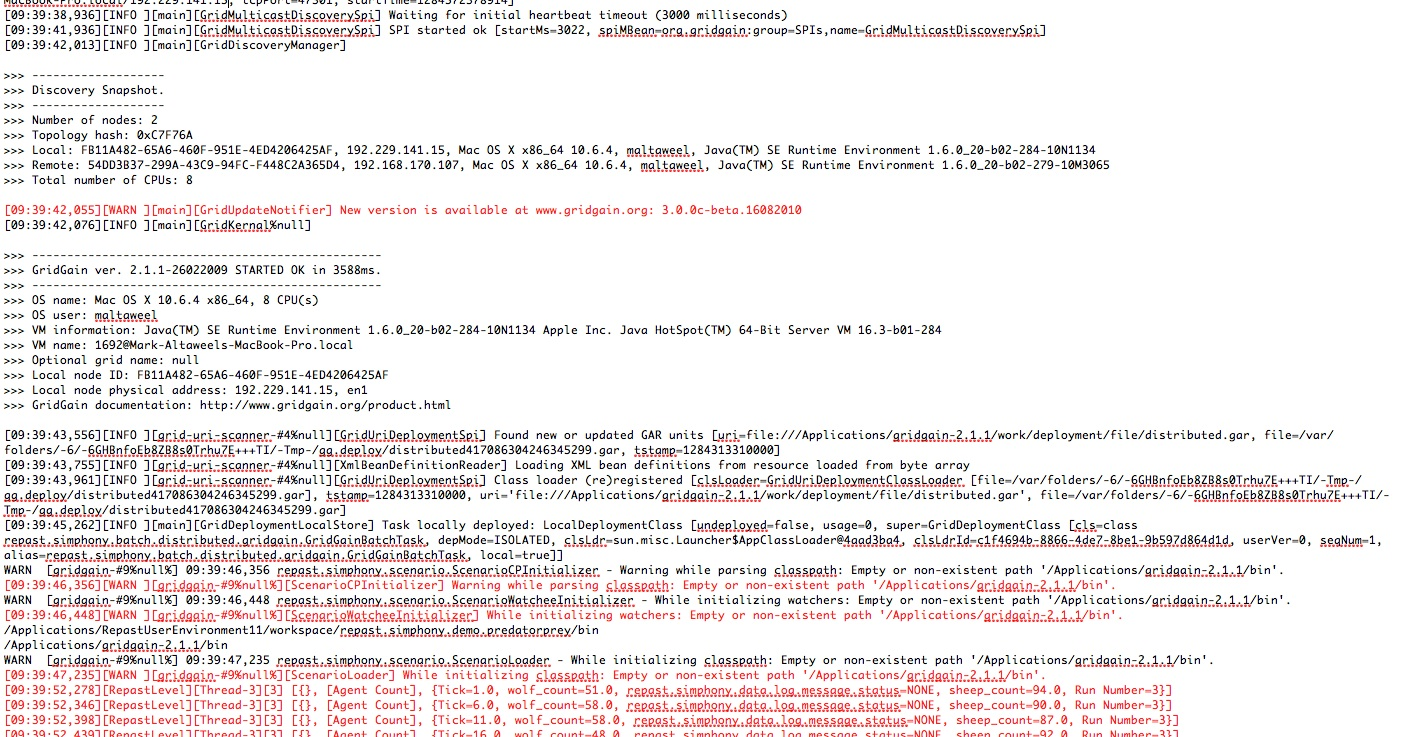
\includegraphics [width=\textwidth]{images/Figure12.jpg}
\label{cablehealth}
\begin{minipage}{.9\textwidth}Figure 12. Local node distributed batch output.
\end{minipage}
\end{center}
\end{figure}

\begin{figure}[!t]
\begin{center}
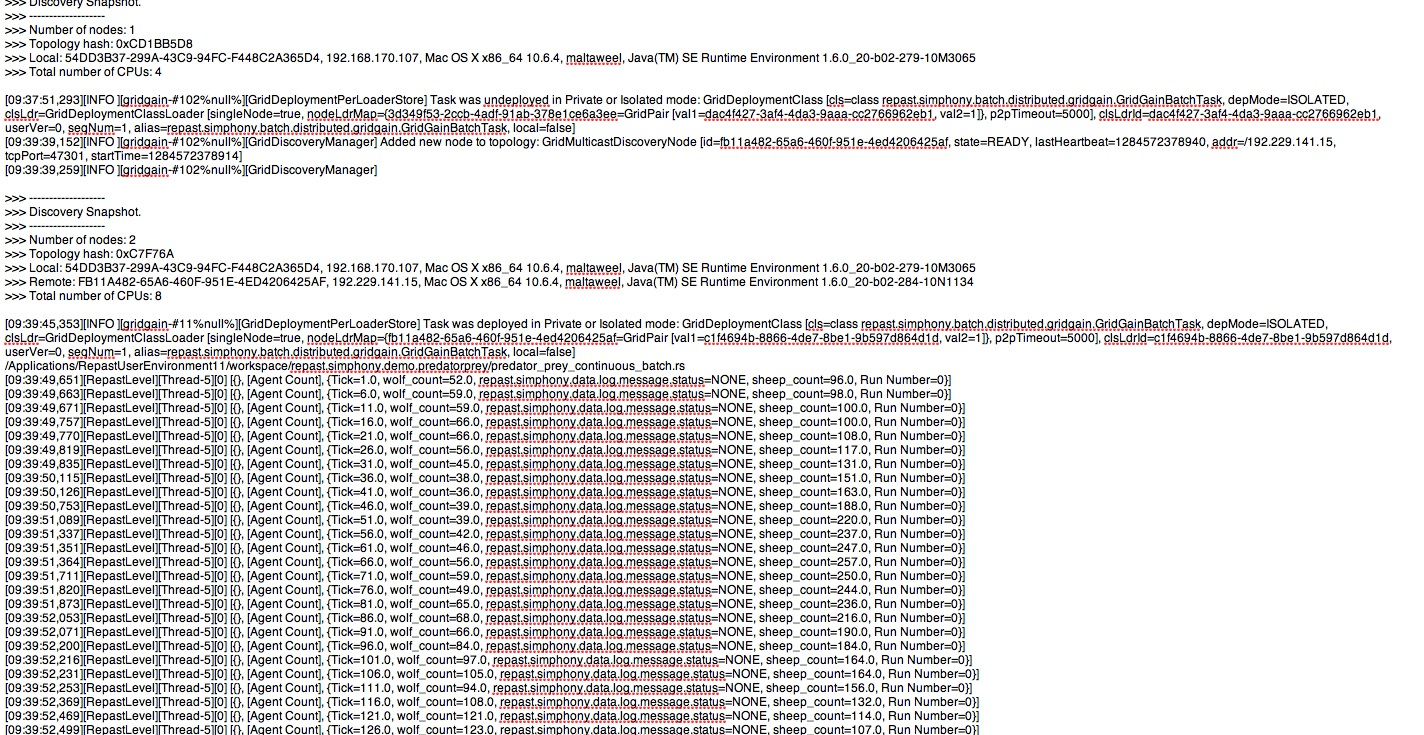
\includegraphics [width=\textwidth]{images/Figure13.jpg}
\label{cablehealth}
\begin{minipage}{.9\textwidth}Figure 13. Remote node distributed batch output.
\end{minipage}
\end{center}
\end{figure}

\section{Outputs Produced}

Outputs produced by the remote and local nodes will be collected and
placed in the /output folder of the users' project (e.g., see
the /output folder in repast.simphony.demo.predatorprey). The output files should be unique for
each run. Remote nodes' outputs that are transferred to the /output
folder may require that the user set a value for the ``delayTime'' parameter in the
XML\_Launch\_Inputs.xml file to enable output results to be transferred to the local node (i.e., the delay would allow enough
time to create the output file and to be transferred over). The local node
may also write local node results to the distributedBatch plugin
path. The user, if desired, can remove these outputs as they will also
be automatically copied over to the /output folder in their project folder. In addition, remote nodes will create output files in the
/bin directories of the GridGain installation on remote nodes. These files are automatically removed if the user
sets the ``removeFiles'' option in XML\_Launch\_Inputs.xml to
``true''. If the user chooses to remove remote output files, these
files will still be transferred to the /output folder in the user's project.

\end{document}
